\documentclass[a4paper,12pt]{article}
\usepackage{amssymb,amsmath}
\usepackage[utf8]{inputenc}

% Setup for fullpage use
\usepackage{fullpage}
\usepackage{graphicx}
\usepackage[ruled,vlined,english]{algorithm2e}
\usepackage{listings}
\usepackage{xcolor}

\usepackage[english]{babel}

\title{
{\Huge Scheduling project}\\
\smallskip
}

\author{
Group member:\\
Vincent Gailly 000547819\\
Maxime Renversez 000545062
\smallskip
}


\date{ Academic year 2021-2022\\
Master in computer sciences \\
\vspace{1cm}
Faculty of sciences, ULB}

\usepackage{amstext} % for \text macro
\usepackage{array}   % for \newcolumntype macro
\newcolumntype{L}{>{$}l<{$}} % math-mode version of "l" column type

\begin{document}
\maketitle
\newpage
\tableofcontents
\newpage

\section{Introduction}

This project is divided into three parts. We have to implement an FTP scheduler, a graphical tool to visualize the results of the scheduling and the Audsley algorithm. In this report, we will explain how we did that. In order to do that, we are going to discuss about the structure of our project, the implementation of the FTP scheduler and Audsley algorithm. We will also provide you an user guide. Before concluding, we will explain the difficulties that we met during the project.      

\newpage

\section{Project structure}
In order to clarify things within the team on how the project was going to be carried out, we made the following class diagram :

\begin{figure}[h!]
  \centering
  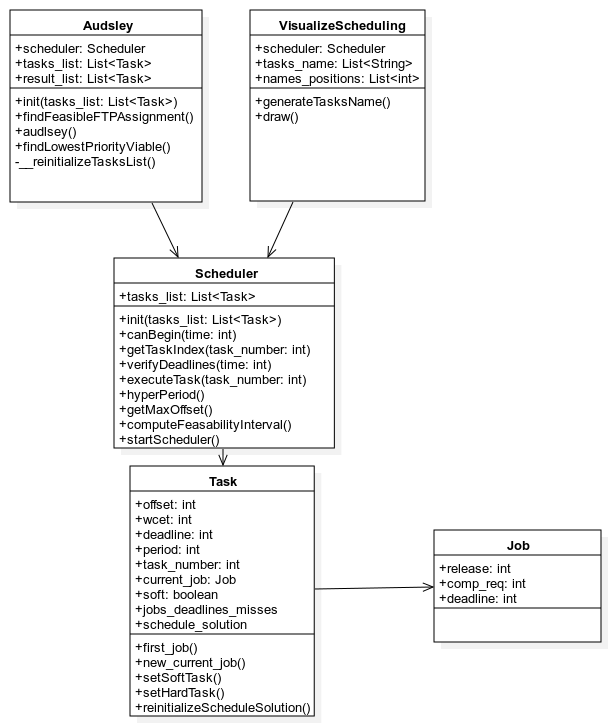
\includegraphics[width=1\textwidth]{Resources_tex/Pictures/audsley.png}
  \caption{Class diagram}
  \label{fig: Project_structure}
\end{figure}

We have decided to do the project in object-oriented programming with Python. We have created different classes wich each represent an object and a file which runs the project. We have created these objects : 

\begin{itemize}
  \item[-] A job is caracterized by a release date, a computationnal time and a deadline.
  \item[-] A task is characterized by an offset, a WCET (Worst Case Execution Time), a deadline, a period, a task\_number (which is used to keep the order with Audsley), a current\_job, a boolean attribute "soft" (True if it is soft, false otherwise) this attribute will allow the Scheduler class to know if it should stop when the task misses its deadline or not, an array jobs\_deadlines\_misses which will allow us to keep a list of the deadlines missed by its jobs and an array schedule\_solution which will contain the solution of the scheduling for this task 
  \item[-] The scheduler has a single attribute “tasks\_list” which is the set of tasks it must schedule 
  \item[-] The class representing the FTP assignment algorithm is Audsley, it is represented by 3 attributes: a scheduler which will allow it to check if a task is lowest priority-viable or not, tasks\_list which represents the set of tasks for which it must find an order, result\_list which will contain the tasks in the order of their priority if the audsley method was able to find a solution. 
\end{itemize}




\newpage

\section{User guide}

In the repository of the project, you use the command : \\
\begin{itemize}
\item[-] python main.py option1 option2
\end{itemize}

\noindent
Where the value of option1 is ``scheduler'' if you want to run the scheduler and display the result. If you want to apply Audsley algorithm, the value of option1 must be ``audsley''. The parameter option2 is a file which contains all the tasks. For example if you run the command : ``python main.py scheduler Tasks.txt''. You obtain the figure 5 as result (see section 4.3). \\
\noindent In the folder ``Tasks'' you can find some set of tasks that have been used for our tests.

\newpage

\section{FTP scheduler}
\subsection{Algorithm}

\definecolor{darkWhite}{rgb}{0.94, 0.94, 0.94}

\lstset{
language=Python,
tabsize=2,
backgroundcolor=\color{darkWhite},
basicstyle=\footnotesize,
breakatwhitespace=false,
breaklines=true,
frame=trbl,
frameround=tttt,
keywordstyle=\color{blue},
commentstyle=\color{red},
numbers=left,
showstringspaces=false
}

\lstinputlisting[language=Python]{
Resources_tex/Code/scheduler.py
}

\smallskip
\noindent
The purpose of this algorithm is to execute the FTP scheduler and returns ``TRUE'' if it ends correctly and ``FALSE'' otherwise. If it returns ``FALSE'' it means that the set of tasks are not schedulable. The variable \textbf{time} represents the current time in the scheduler. The variables \textbf{job\_duration} and \textbf{job\_start} represent the duration of the execution of one job and at which time the job is executed for the first time (these variables allow us to keep a track of the execution of all the jobs of all the tasks). The variable \textbf{task\_number} is the number of the task which has its job that is being executed (if the task which executes its job first is not the task 1 it is not a problem because in the list of solution for the task 1 we add the tuple ``(0,0)'') . The variable \textbf{feas\_int} represents the upper bound of the feasibility interval which is calculated by the method ``computeFeasibilityInterval()''. The while loop will be explained in subsection 4.2. The condition at the line 29 allows to add the execution of the job of the task which was executed when a deadline was missed in the list of solutions of the task.

\subsection{Explanations of the while loop}

To stay in the loop, two conditions must be respected : \\
\begin{itemize}
\item[-] The time must be less or equal to the upper bound of the feasibility interval.
\item[-] No deadlines are missed. 
\end{itemize}

\smallskip
\noindent
When the program enters in the loop, it first calculates which task can execute its job and stores its number in the variable \textbf{task\_to\_execute}. It is done by the method ``canBegin(time)'' which takes the current time in parameter and returns a task number. This method respects the task priorities. For example, if two tasks can execute their job at the same moment, it returns the task number which has the higher priority. But if no tasks can execute a job (it is when all the jobs have finsihed their executions and the new jobs are not yet released), it returns ``-1''. Once we know which task can execute its task, we must dinstinguish four cases. Before explaining these cases, just a reminder of the difference between \textbf{task\_number} and \textbf{task\_to\_execute}. We can see the first one as the ``past'' (at time t-1) and the second one as the ``present'' (at time t).

\subsubsection{Case 1}

\begin{figure}[h!]
  \centering
  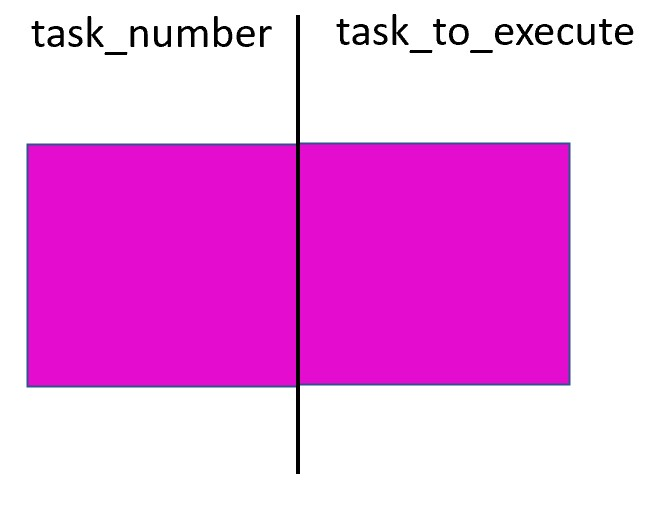
\includegraphics[width=0.5\textwidth]{Resources_tex/Pictures/Case1.jpg}
  \caption{Case 1}
  \label{fig: Case 1}
\end{figure}

\smallskip
\noindent
It is the case when the job executed at time t-1 is the same as the job executed a time t (see lines 22 - 23 in the algorithm). It is the easiest case. Indeed, we just need to increment the duration of the execution of job because the job will be executed one more unit of time. 


\newpage

\subsubsection{Case 2}

\begin{figure}[h!]
  \centering
  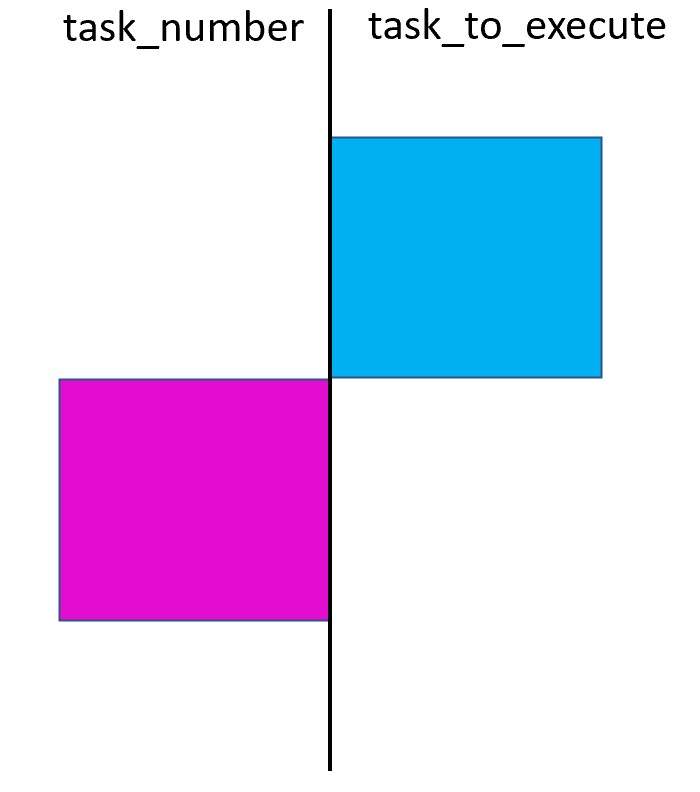
\includegraphics[width=0.5\textwidth]{Resources_tex/Pictures/Case2.jpg}
  \caption{Case 2}
  \label{fig: Case 2}
\end{figure}

\smallskip
\noindent
It is the case when at time t-1 the job of a task is executed and at time t the job of another task is executed (sees line 16 - 18 in the algorithm). In this case, we add a tuple composed of the start time of the job (given by the variable \textbf{job\_start}) and its duration (given by the variable \textbf{job\_duration}) in a list belonging to the task whose the job was executed at time t-1. We reset the value of the two variables (\textbf{job\_start} = time and \textbf{job\_duration} = 0) for the job which will be executed at time t. 

\newpage
\subsubsection{Case 3}

\begin{figure}[h!]
  \centering
  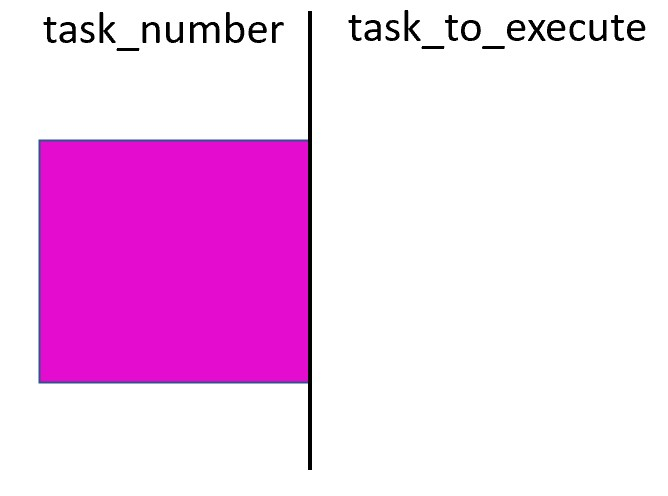
\includegraphics[width=0.5\textwidth]{Resources_tex/Pictures/Case3.jpg}
  \caption{Case 3}
  \label{fig: Case 3}
\end{figure}

\smallskip
\noindent
It is the case when a time t-1 the job of a task ended and a time t, there is no tasks that can execute their job (see lines 28 - 30 in the algorithm). So the value of \textbf{task\_number} is the task number which has its job executed at time t-1 and \textbf{task\_to\_execute} is -1 (because no tasks can execute their job). In this case, we add a tuple composed of the start time of the job (given by the variable \textbf{job\_start}) and its duration (given by the variable \textbf{job\_duration}) in a list belonging to the task whose the job was executed at time t-1. We also set the values of \textbf{job\_duration} and \textbf{job\_start} at 0.

\subsubsection{Case 4}

\begin{figure}[h!]
  \centering
  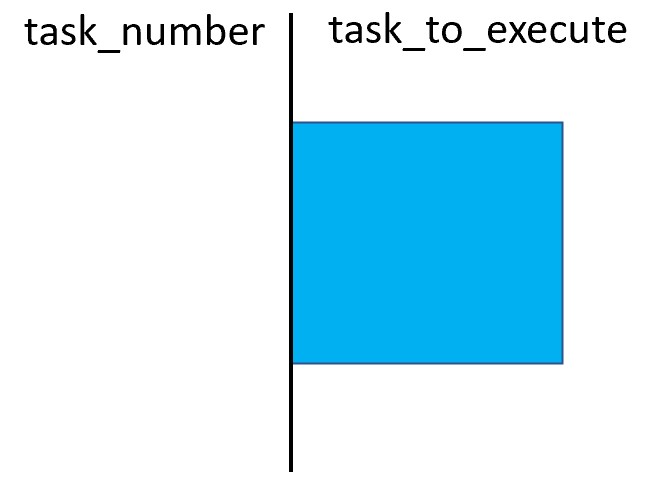
\includegraphics[width=0.5\textwidth]{Resources_tex/Pictures/Case4.jpg}
  \caption{Case 4}
  \label{fig: Case 4}
\end{figure}

\smallskip
\noindent
It is the case when no job is executed at time t-1 (it means that the value of \textbf{task\_number = -1}) and a job can be executed a time t (it means that the value of \textbf{task\_to\_execute} is the number of the task which can execute its job). We just need to set the values of \textbf{job\_start} at time t and \textbf{job\_duration} at 1 (see lines 20 - 21 in the algorithm) because a new job starts its execution.

\subsubsection{Case 5}
If the values of \textbf{task\_number} and \textbf{task\_to\_execute} are -1, we do nothing (see line 26 in the algorithm). 

\newpage
\subsection{Result of an execution}

Consider that we have four tasks to schedule and they are ordered by priority : \\

\smallskip
\begin{center}
\begin{tabular}{| l |}
\hline
Task 1 (Offset = 0, WCET = 10, Deadline = 50, Period = 50)\\
Task 2 (Offset = 0, WCET = 20, Deadline = 80, Period = 80)\\
Task 3 (Offset = 0, WCET = 10, Deadline = 100, Period = 100)\\
Task 4 (Offset = 0, WCET = 50, Deadline = 200, Period = 200)\\
\hline
\end{tabular}
\end{center}

\smallskip
\noindent
Thus the priority of the tasks is : Task 1 $>$ Task 2 $>$ Task 3 $>$ Task 4. \\

\noindent
The result of the scheduling is : \\

\begin{figure}[h!]
  \centering
  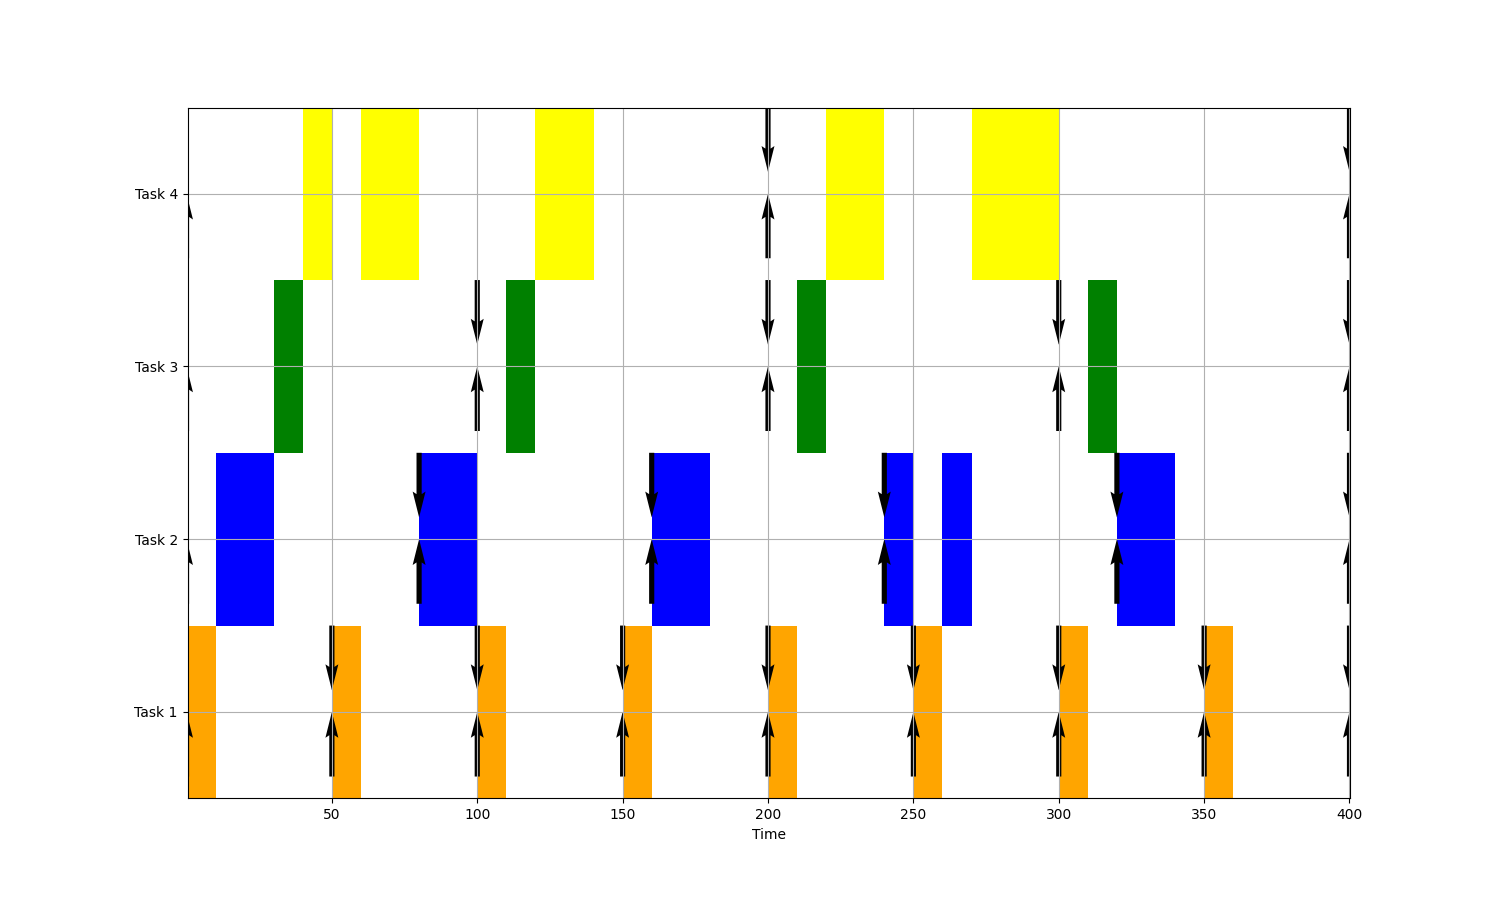
\includegraphics[width=1\textwidth]{Resources_tex/Pictures/Figure_1.png}
  \caption{Scheduling 1}
  \label{fig: Scheduling 1}
\end{figure}
\noindent
The arrow $\uparrow$ is when a job can start its execution and the arrow $\downarrow$ is the deadline of a job. 

\newpage 
\noindent
But what happens if a deadline is missed ? Consider the following task : \\
\begin{center}
\begin{tabular}{| l |}
\hline
Task 1 (Offset = 0, WCET = 30, Deadline = 25, Period = 60)\\
\hline
\end{tabular}
\end{center}
This task will always miss its deadline. The result of the scheduling is :\\

\begin{figure}[h!]
  \centering
  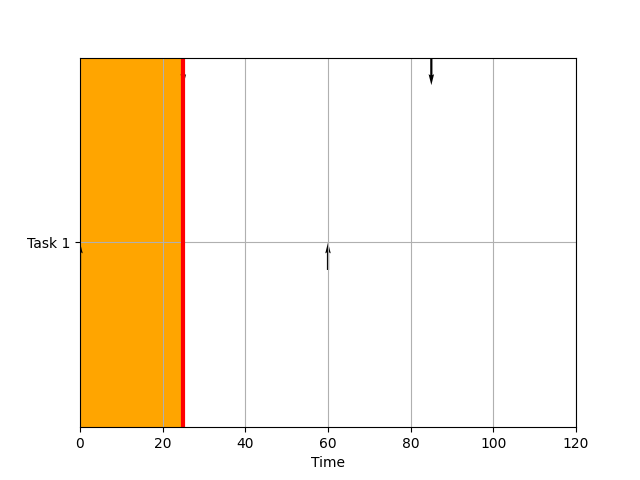
\includegraphics[width=1\textwidth]{Resources_tex/Pictures/Figure_2.png}
  \caption{Scheduling 2}
  \label{fig: Scheduling 2}
\end{figure}
\noindent
 The read line shows that the deadline is missed. 
 
\newpage
\section{Audsley’s priority assignment}
Audsley's algorithm is based on the following theorem "Suppose that $\tau_i$ is lowest-priority viable. Then, there exists a feasible FTP-assignment for $\tau$ iff there exists an FTP-priority assignment for $\tau\backslash \{\tau_i\}$." \\

\smallskip
\noindent
In this theorem it is mentioned the notion of lowest-priority viable. A task is said to be lowest-priority viable if it can complete all its jobs before they meet their deadlines, while having a lower priority than the other tasks that must be scheduled and that the other tasks are considered as "soft".\\

\smallskip
\noindent
To implement this algorithm, we had to do it recursively. Indeed, we had to find in the list of tasks given as inputs a lowest priority-viable task, once found this one was added at the end of the table which contains the list of tasks in the order of priority and was not considered anymore to find the next lowest priority-viable.\\

\lstinputlisting[language=Python]{
Resources_tex/Code/audsley.py
}

\smallskip
\noindent
This piece of code can be divided into 3 parts: 

\begin{itemize}
  \item[-] the first if will handle the case where there is only one task left, in this case you don't have to search after a lowest priority-viable, you just have to check that the last task is schedulable. (i.e. the deadline is smaller than the WCET)
  \item[-] the second one returns false in case none of the tasks can be lowest priority-viable in the remaining set of tasks
  \item[-] the else recursively calls the method but removing the lowest priority-viable found with the "findLowestPriorityViable()" method from the set of tasks
\end{itemize}

\newpage
\lstinputlisting[language=Python]{
Resources_tex/Code/find.py
}

\smallskip
\noindent
In the above code, we will start by going through the tasks\_list with a for loop and consider the element of the first loop as the lowest priority-viable, then a second loop will set the other tasks to "soft" and insert them in the temporary list. \\
The task we will try as LPV will be set to "hard" and at the end of this second loop we will add the potential lowest priority-viable at the end of the temporary list in order to give it the lowest priority. \\
Then we will launch the scheduler with the set of tasks set in order of priority and we will check that no deadline has been missed by the hard tasks. If this is the case we continue the for loop, otherwise we insert the LPV in the result\_list attribute and remove it from the tasks\_list. We will also reset the tasks\_list and return True. \\
This method returns False when the first for loop stops and it has not found any LPV.
\newpage

\section{Difficulties}

The first difficulty that we have met, is to create the visualize tool. We did not know which type of graphic to choose to represent the solution. We have decided to work with Gant diagrams. After that, we have read the documentation of the function that allows to do this kind of diagram. The method requires two arguments : a list of tuples (A,B) and a tuple composed of the minimum ``y'' coordinate and the maximum ``y'' coordinate. The ``A'' is the x coordinate of the start of the rectangle that will be drawn by the function and ``B'' is the size of the rectangle. Once we knew that, we had to find a way to keep track of the execution of the job (when they started and the duration of their executions). In order to do that, we have create a parameter for each tasks that allow us to save these informations. \\

\smallskip
\noindent
Once we had our visual tool, we started to test our scheduler. We noticed some errors. In order to solve them, we thought about the different possible cases (we explain these cases at section 4.2). As soon as our scheduler worked well, we started to implement the Audsley algorithm. The implementation of this algorithm was not a problem for us because we understood well how its works. The only two problems that we met with this algorithm was that we forgot to set the tasks as hard tasks after each iterations (in order to find the lowest priority viable variable) and thus the priority assignment was always wrong. The second problem was about our solution. When we found a lowest priority viable variable, we inserted it with the method ``insert(-1,the task)'' and therefore our order was always wrong (the solution was to replace the -1 by 0). 

\newpage

\section{Conclusion}
This project was very interesting and allowed us to learn more about scheduling. \\
The fact that we had to implement a scheduler ourselves made us think about the many cases we could come across and how to deal with them. \\
We were also able to discover more in depth the Audsley algorithm and the logic behind it to assign priorities to a set of tasks in an efficient way.

\end{document}